%!Mode:: "TeX:UTF-8"
\section{Procfs和Sysfs}

\subsection{Procfs}
在许多类 Unix 计算机系统中, procfs是进程文件系统 (file system) 的缩写,包含一个伪文件系统(启动时动态生成的文件系统),用于通过内核访问进程信息。这个文件系统通常被挂载到 /proc 目录。由于 /proc 不是一个真正的文件系统,它也就不占用存储空间,只是占用有限的内存。

The proc file system acts as an interface to internal data structures in the kernel. It can be used to obtain information about the system and to change certain kernel parameters at runtime (sysctl).
The proc filesystem provides a method of communication between kernel space and user space. For example, the GNU version of ps uses the procfs to obtain its data, without using any specialized system calls.

task目录就是用来描述进程中线程的,因此也可以通过下面的方法获取某进程中运行中的线程数量(PID指的是进程ID):
\begin{verbatim}
ls /proc/PID/task | wc -l
\end{verbatim}  


\subsection{Sysfs}
Sysfs 是 Linux 2.6 所提供的一种虚拟文件系统。这个文件系统不仅可以把设备(devices)和驱动程序(drivers) 的信息从内核输出到 用户空间,也可以用来对设备和驱动程序做设置。
当时由于procfs 文件系统过度混乱,包含了许多不是进程(process)的信息, sysfs 的目的是把一些原本在 procfs 中的,关于设备的部份独立出来,以‘设备层次结构架构’(device tree)的形式呈现。
每个被加入 driver model tree 内的对象,包括驱动程序、设备以及 class 设备,都会在 sysfs 文件系统中以一个目录呈现。

Sysfs通常被加载到/sys目录。

\begin{figure}[ht]
	\begin{center}
		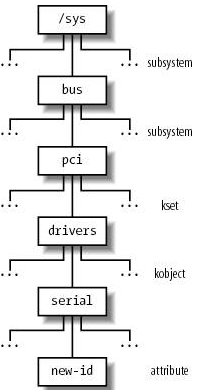
\includegraphics[keepaspectratio,width=0.3\paperwidth]{Pictures/Kernel/DeviceDriverModelHierarchyExample.png}
	\caption{驱动程序模型层次}
	\label{fig:DeviceDriverModelHierarchyExample}
	\end{center}
\end{figure}

sysfs 一开始以 ramfs 为基础,也是一个只存在于存储器中的文件系统。sysfs 刚开始被命名成 ddfs (Device Driver Filesystem),当初只是为了要对新的驱动程序模型除错而开发出来的。它在除错时,会把设备架构(device tree)的信息输出到 procfs 文件系统中。但在 Linus Torvalds 的急切督促下,ddfs 被转型成一个以 ramfs 为基础的文件系统。在新的驱动程序模型被集成进 2.5.1 核心时,ddfs 被改名成 driverfs,以更确切描述它的用途。在2.5 核心开发的次年,新的“驱动程序模型”和 "driverfs" 证明了对核心中的其他子系统也有用处。kobjects 被开发出来,作为核心对象的中央管理机制,而此时 driverfs 也被改名成 sysfs。



\clearpage